\chapter{Formalizing and automating the release process}

\label{chap:release}

\section{Introduction}

The process of releasing new software versions is a crucial part of software development that directly affects how users will be able to benefit from it.
It is related to the questions of compatibility between versions, of reactivity of bug fixing (because a bug fix is only useful to most users when it is eventually released), and of documentation (so that users can read about the things they need to be aware of before upgrading).
Software that is not released for a long time will become incrementally less useful to its users~\cite{lehman1996laws} and may be viewed by them as dead.
Software that receives large breaking changes, or where some of the breaking changes are not documented, can prevent users from upgrading, or at least significantly delay the process.
Finally, well-thought and understandable version numbering schemes are as important as documentation~\cite[Chapter~7]{fogel2005producing} in a world where software projects have more and more dependencies~\cite{decan2019empirical}.

As observed by Michlmayr~\cite{michlmayr2007thesis}, release management is generally not an issue for young projects.
They tend to release frequently, because getting user feedback is critical, and the release process is generally simple.
Today, lots of conventional wisdom and tooling is available to help them: standardized versioning semantics~\cite{preston_semantic_versioning}, a standardized changelog format~\cite{keep_a_changelog}, automatic changelog generators~\cite{conventional_changelog}, continuous integration and deployment services~\cite{appveyor,azure_pipelines,circleci,gitlab,travisci}, release notes and artifact sharing mechanisms~\cite{github_releases}, ecosystem-specific package managers (cf. Chapter~\ref{chap:distribution}), etc.

However, as projects mature and grow larger, releases tend to be produced less frequently.
The seven projects that Michlmayr studied in his thesis~\cite{michlmayr2007thesis} had all experienced significant delays in producing releases before they decided to switch to time-based release cycles.

Longer time between releases creates a number of problems, and a switch from feature-based to time-based release cycles is generally expected to solve them, resulting in: shorter time for users to benefit from new features and fixes, and thus shorter feedback loop for developers, less disruption between two successive releases, better planning and no ``last-minute feature rush''~\cite{fogel2005producing} (or ``thundering herd of patches'' to reuse the expression of kernel developer Ted Ts'o~\cite{corbet2002kernel}) because missing a release is not a big deal if the next one is coming shortly after.

However, switching to short release cycles comes with a number of associated challenges, to make the release process efficient and lightweight enough.
After a historical presentation of the switch to time-based releases in the Coq project, I present some challenges that this created, and how I contributed to solve them.
Beyond the challenge of continuous testing that was addressed in Section~\ref{sec:ci}, the three main challenges presented in this chapter are: how to separate the contributing process from release management; how to streamline the backporting process; how to prepare consistent release notes.

While the complex release strategies of large open source projects are already well documented~\cite{gcc_dev_plan,erenkrantz2003release,rahman2015release,khomh2012faster,jorgensen2001putting}, and short release cycles have now been largely studied~\cite{cesar2017frequent}, my contribution should be useful to medium-sized projects, which have overgrown what standard recommendations and tools can help them do, without having reached the size nor requiring the process complexity of the biggest open source projects which have been the focus of most research so far.

\section{Historical overview: towards more frequent releases}

\label{sec:frequent-releases}

Until the release of Coq 8.5, the frequency of new releases used to vary a lot (cf. Table~\ref{tab:releases}), depending on the features that were planned for the release: Coq 8.5 was released three and a half years after Coq 8.4, which was released two years after Coq 8.3, which was released one and a half year after Coq 8.2.
The period of beta testing, separating the first beta release from the final release was frequently above six months, even rising to a full year in the case of Coq 8.5.

Under the impulse of Maxime D\'en\`es, Coq adopted time-based, shorter release cycles, starting with Coq 8.6, which was released 11 months after Coq 8.5, Coq 8.7, which was released 10 months after Coq 8.6, and Coq 8.8, which was released just 6 months after Coq 8.7.
An official release manager was appointed (initially Maxime D\'en\`es; and since Coq 8.9 it has become a rolling position); feature freeze dates were set by the release manager, instead of waiting for the completion of the planned features; beta releases were shortened thanks to continuous testing of the master branch (cf. Section \ref{sec:ci}).

\begin{table}
	\begin{center}
		\begin{tabular}{|c|c|c|c|}
			\hline
			Major releases & Release dates & Time since previous release & Duration of beta-testing \\
			\hline
			8.2 & 2009-02 & -- & 8 months \\
			\hline
			8.3 & 2010-10 & 20 months & 8 months \\
			\hline
			8.4 & 2012-08 & 22 months & 8 months \\
			\hline
			8.5 & 2016-01 & 41 months & 12 months \\
			\hline
			8.6 & 2016-12 & 11 months & 1 month \\
			\hline
			8.7 & 2017-10 & 10 months & 1 month \\
			\hline
			8.8 & 2018-04 &  6 months & 1 month \\
			\hline
			8.9 & 2019-01 &  9 months & 2 months \\
			\hline
			8.10 & 2019-10 & 9 months & 5 months \\
			\hline
		\end{tabular}
		\caption{
			Dates of major releases since 8.2, with final release dates, elapsed time since the previous final release date, duration between the first beta release and the final release (the stabilization period is in fact longer).
			Source: \url{https://coq.inria.fr/news/}.
		}
		\label{tab:releases}
	\end{center}
\end{table}

Coq has also adopted dot-separated three-digit version numbers corresponding to the standard scheme~\cite[Chapter 7]{fogel2005producing}, which is used in particular in semantic versioning~\cite{preston_semantic_versioning}, except that it does not (at least it does not yet) follow the semantics of semantic versioning (both first numbers indicate major releases, there are no minor releases, the last digit does indicate patch-level releases).\footnote{
	The scheme that was used previously in the Coq 8 series was 8.XplY where 8.X was the major version number, and Z was the patch-level number.
	This scheme had been adopted from other projects (in particular PHP projects) using it (source: \url{https://github.com/coq/opam-coq-archive/issues/8}).
}
Patch-level releases have also been released more frequently (every two to four months) since Coq 8.7.

Overall, the adoption of shorter release cycle has successfully managed to provide more stable versions, with less breaking changes, that are easier to upgrade to (see also the compatibility policy described in Section~\ref{sec:compatibility-policy}).
In-depth evaluations of the time it takes for feature or bug fixes to reach users, similar to what was done by da Costa \emph{et al.}~\cite{da2018impact}, or of the cumulated effort users invest in porting their projects to new versions of Coq over many years, would be worthwhile, but have not been conducted as of today.
However, the switch to shorter release cycles also imposes efficiency constraints, and this is what this chapter is about.

\section{How to separate contributing from release management?}

\subsection{Branching strategy}

Branches are a wonderful feature of modern version control systems (VCS) that allow project owners to manage several versions of a code base in parallel.
We generally distinguish two kinds of branches.
Topic branches are short-lived branches that developers use to work on a specific topic (such as a new feature or a bug fix): they are the base ingredient of pull-based development.
On the other hand, a limited number of long-lived main branches (at least one) is maintained by a project to manage different versions of the software: one of them is usually distinguished and called ``master'' in the Git terminology, or ``trunk'' in the SVN terminology.
In this section, I am focusing specifically on how these main branches are managed.

In small open source projects, it is quite frequent to have a single maintainer that takes care of the integration of pull requests and the preparation of new releases, or to have a small team of maintainers that work together to make sure that changes are integrated, and new versions are released according to a shared plan.
For small software projects, such as software libraries, releasing a new version may be as simple as publishing a new tag and a changelog.
In these cases, branch management may be easy: the project maintains a single public branch, usually called master, from which all new versions are tagged.
Even patch-level releases can be prepared from the master branch, as long as no new feature has been integrated since the last release.

Because releases are cheap, patch-level releases frequently include just a few bug fixes (sometimes just one).
Besides, because minor releases are easy to upgrade to, when the project follows semantic versioning, maintainers will usually not bother releasing a patch-level version for a fix that has been integrated \emph{after} a feature, unless the bug is considered of critical importance (typically security fixes).

In a study of 2,923 GitHub projects (selected for having five-year of active history, at least 100 commits, 3 contributors, one closed pull request, and excluding forks and non-software projects), Zou \emph{et al.}~\cite{zou2019branches} found that 18\% of selected projects only use a single branch.
Among the projects that use multiple branches, they found that about 25\% of the non-master branches are used for version iteration (i.e. what is usually designated as \emph{release branches}), the rest can be considered topic branches.
Unfortunately, they did not compute the proportion of projects that use release branches.

For larger projects with many contributors, new features are prepared, reviewed, and ready to be integrated all the time.
Stabilization in preparation of a new release may require coordination through a feature freeze (a period during which no new features may be integrated).
This is what is done in the GCC project for instance~\cite{gcc_dev_plan}.
A first release candidate is published at the end of the feature freeze.
At this time, a new release branch is created.
This release branch will make it possible to prepare patch-level releases without preventing the integration of new features in the master branch.

In the Coq project, in order to make it possible to involve a larger group in the pull request integration process (cf. Section~\ref{sec:distributed-merging}), we proceed slightly differently to handle the stabilization phase leading to a first beta release.
What we call erroneously a feature freeze is in fact a cutoff date at which time a new release branch is created (from the current state of the master branch).
This release branch will be where the stabilization phase will take place, under the authority of the release manager, which is the only person allowed to update this branch (and whom we should call the ``release owner'' according to Fogel's definition~\cite[Chapter 7]{fogel2005producing}).
This means that the integration of new features in the master branch never stops, so integrators do not have to care or even be aware of the release schedule.
Meanwhile, it may take a month or more before a first beta version is finally released.
No release is ever done from master.%
\footnote{Although the master branch still receives specific ``alpha'' tags marking the first commit to \emph{not belong} to a given stable version, and thus the beginning of the development of the next one.}

This workflow was made possible by a change in branch management, that occurred previously under my conduct.

\subsection{Inverting the patch-porting workflow}

The previous model (that was used from January 2015 to July 2017) was similar to the one that is used today in the Symfony project~\cite[Section ``Choose the right Branch'']{symfony_pull_request}, except that it was not formalized nor documented.
Bug fixes had to target a release branch (the earliest branch in which the developer wanted the fix to be applied), and release branches were subsequently merged into more recent release branches, all the way up to the master branch.
This process had several issues: bug fixes took longer to reach the master branch, which some users used as their working version of Coq; and contributing was made more difficult by having to choose on which branch to prepare a pull request.\footnote{See for instance \url{https://github.com/coq/coq/pull/463}, \url{https://github.com/coq/coq/pull/495}, \url{https://github.com/coq/coq/pull/538} (bug fixes that initially targeted the master branch) and \url{https://github.com/coq/coq/pull/90}, \url{https://github.com/coq/coq/pull/191} (features that initially targeted a release branch).}
Despite the thorough contributing documentation that Symfony provides, they suffer from the same issue.\footnote{
	Here is a hand-picked selection of pull requests that did not target the right branch from the start, and had to be rebased from August 5\textsuperscript{th} to August 16\textsuperscript{th}, 2019: \url{https://github.com/symfony/symfony/pull/32947}, \url{https://github.com/symfony/symfony/pull/32977}, \url{https://github.com/symfony/symfony/pull/33093}, \url{https://github.com/symfony/symfony/pull/33151}, \url{https://github.com/symfony/symfony/pull/33199}.
}

The new process uses backporting~\cite{hua2014case} instead: pull requests should virtually always target the master branch, and they are cherry-picked (i.e. automatically reapplied) to stable release branches when they satisfy the criteria for inclusion.
This process solves the issues of the previous model: fixes are immediately available in master, and contributors do not have to worry about which branch to target.
Furthermore, because the backporting process occurs \emph{after} a pull request has been merged, the release manager can reject some proposed changes without requesting anything from the pull request author.
Thus, it makes it less likely that they will have to bear a debate on the acceptability of the patch every time this happens, nor have to sound dictatorial.

The new process was introduced at the time the release branch for Coq 8.7 was created.
From this time, all pull requests should be merged in the development branch, unless they are specific to a release branch.
Only the person in charge of the release branch (initially myself for the release branches of Coq 8.7 and 8.8, a period during which Maxime D\'en\`es and I shared some responsibilities of release management, then the appointed release manager starting with Coq 8.9 when it became a rolling position) can push to the release branch.

\section{How to streamline the backporting process?}

\label{sec:backporting}

\subsection{Visualizing the backporting tasks}

A common issue in projects that rely on backporting, especially in the absence of a clear and formalized process on what gets backported and who does it, is that some commits get backported when they should not have, and some commits do not get backported when they should have.
A previous study on backporting in the Linux kernel~\cite{hua2014case} found that, while only experts are tasked with backporting activities, a significant proportion of them still finds it a hard and error-prone process.
Recently, machine-learning tools have been designed to select patches for automatic backporting~\cite{edge2018machine,hoang2019patchnet,wen2019ptracer}, but it has sometimes led to patches introducing regressions getting backported nonetheless~\cite{corbet2019linux}.

I implemented a process whose goal is to avoid these kinds of issues, and which I adapted based on the feedback I received during the first few weeks of its application.\footnote{
	Cf. \url{https://gitter.im/coq/coq?at=596dfff82723db8d5e217283} and \url{https://gitter.im/coq/coq?at=598c0281329651f46e079a36}.
}
The process relies on milestones, and a ``GitHub project''.
``Projects'' are a GitHub feature that was announced in 2016~\cite{github_projects_announcement}, which allows to create a Kanban-like board with columns that can contain notes, issues, and pull requests.

Before merging a pull request, the pull request assignee must choose a milestone (and is reminded to do so by the merging script, see Section~\ref{sec:distributed-merging}).
Most of the time, the choice is between the upcoming version of the release branch (which may be a beta version, a ``final'' version, or a patch-level version) and the version under active development.
This gives an indication of intent, but ultimately it is the decision of the release manager to follow the indication, or to edit the milestone.
It is similar to the tag \verb|stable@vger.kernel.org| that patch authors or integrators can use in commit messages to signal backporting intent to stable kernel maintainers.

When a pull request is merged into the milestone corresponding to the next stable release, the pull request is added to a ``Request inclusion in ...'' column in the project board.
Then the release manager selects some pull requests to backport, and does it using a backporting script (that automatically cherry-picks the pull request commits onto the release branch).
The batch of backported pull requests is generally pushed to a branch so that CI can run.
When backported pull requests are finally pushed to the release branch, they are moved to a ``Shipped in ...'' column.

The use of a GitHub project board makes the backporting process both non-invasive, and transparent.
Kerzazi and Robillard~\cite{kerzazi2013kanbanize} also report on the use of a Kanban-inspired release process, and although the use of the Kanban board is different (it is used actively by multiple developers, and is used for the whole release process instead of specifically the backporting process like here), one of their first motivating issue, ``lack of visibility on the release process'', is similar.

\subsection{Automation}

At first, I used this process and managed the project board manually, using filters to find which pull requests needed to be added to the first column.
Then GitHub added simple automation to project boards~\cite{github_project_automation}, which despite being too simple for the kind of workflow I was using, still inspired me to automate the management of pull requests within the backporting board.
I implemented this automation in the bot (presented in Section~\ref{sec:bot}).

It is triggered by any pull request, push, and project board event.
When a pull request is merged on master, it checks whether the description of its milestone contains an indication of a column to add the pull request to.
If it is the case, it adds it there.
When a pull request is backported to a release branch, it looks again at the description of the milestone to see to which column it should move the corresponding card (see Figure~\ref{fig:backport}).

Finally, when a pull request is removed from a project board, it checks the milestone description to see if it was removed from a ``Request inclusion ...'' column corresponding to its milestone, and if it is the case, it updates the pull request milestone to the one of the version under development, and posts a message informing the stakeholders that the pull request was postponed (see Figure~\ref{fig:reject-backport}).

\begin{figure}
	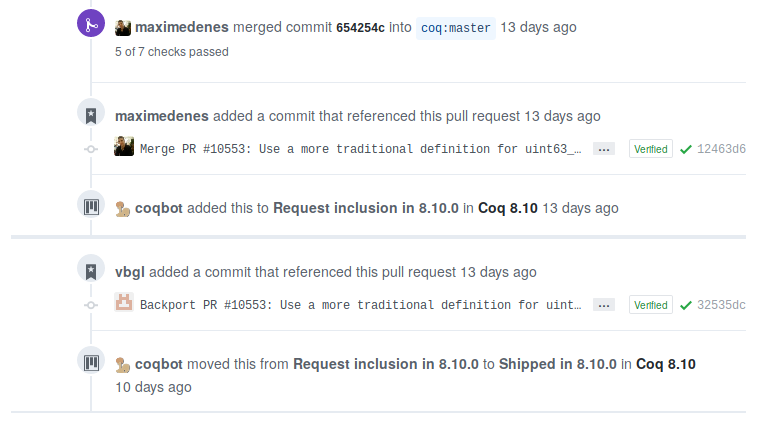
\includegraphics[width=15cm]{backport-management.png}
	\caption{
		A screenshot of a pull request getting merged, automatically added to the backporting project, and getting backported by the release manager (of Coq 8.10).
	}
	\label{fig:backport}
\end{figure}

\begin{figure}
	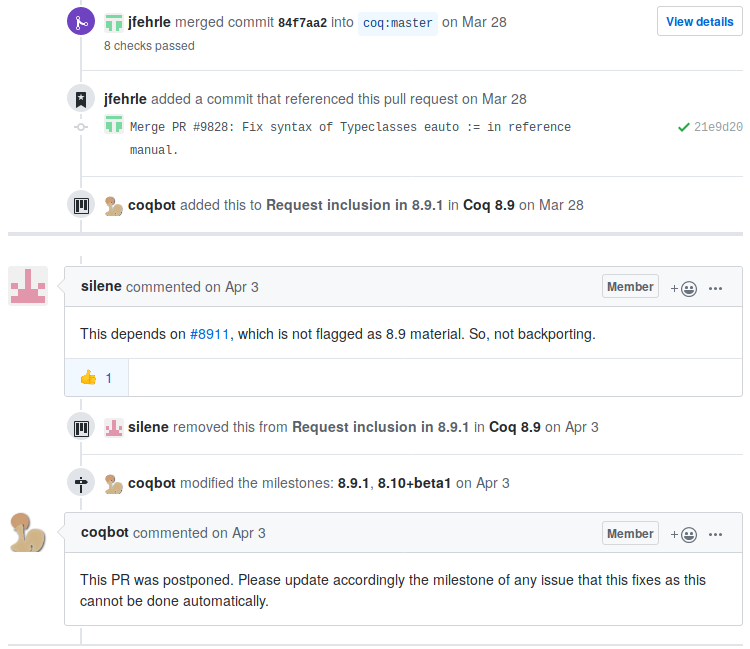
\includegraphics[width=15cm]{reject-backport.png}
	\caption{
		A screenshot of a pull request whose backporting is rejected by the release manager (of Coq 8.9).
		In this case, the release manager took the time to explain the decision, but when that is not the case, the automatic message from the bot is useful so that stakeholders are informed.
	}
	\label{fig:reject-backport}
\end{figure}

\subsection{Open issues, future work}

\label{sec:open-issues-backport}

The current workflow has a known limitation that will need to be addressed in the future.
Some more automation could also be implemented.

The main limitation to the use of milestones to suggest backporting is that a pull request can have at most a single milestone.
The presented workflow is thus not well suited to maintaining several release branches at the same time.
Currently, the Coq project does not maintain old stable versions (producing new patch-level releases after a more recent stable version has been released).
However, it can happen that the last patch-level release of the current stable version is still in preparation while the branching and stabilization process for the next stable version has already started.
In this case, it can happen that a pull request should be backported to the two active release branches.

Up to now, such cases have been infrequent enough to be managed manually.
However, formalizing and automating this part of the workflow as well would ensure that accidental mistakes do not occur.
In particular, a mistake would be for the release manager of the current stable version to backport a fix and publish a new patch-level release which incorporates it, but for the release manager of the upcoming stable version to miss this fix and not backport it.
This would then create a regression, because users updating from one version to the next (both semantically and chronologically) would discover that the bug that was fixed is back.

Possible improvements to the automation include: creating automatically the backporting project board; managing the case of pull requests that were not marked for backporting but the release manager decides to backport nonetheless; not posting an automatic comment when the release manager has rejected a pull request but has just posted a comment explaining why; automatically running the backporting script for the pull requests that can be cherry-picked without conflicts, so that the CI results are already available, and the release manager can just approve or reject them.

\section{How to prepare consistent release notes?}

\label{sec:release-notes}

\subsection{Changelog and release notes in software development}

Keeping a changelog is considered to be an important quality criterion in software development.
Comprehensive and understandable release notes are especially useful to preexisting users of a software product, as it will help them understand what differences they should expect in the new version, especially what are the incompatibilities, the new features, and the bug fixes (possibly only the most important ones if the list is too long).

Several attempts have been made to formalize how a changelog should be kept~\cite{gnu_changelog,keep_a_changelog}.
In particular, the ``Keep a Changelog'' initiative, started in 2014, and whose version 1.0.0 was published in 2017, has been quite successful among projects hosted on GitHub, since searching for files whose name is exactly \verb|CHANGELOG.md|, and which contain the words ``The format is based on Keep a Changelog'' yields 200,000 results.

There are also initiatives to automate the generation of release notes based on commit messages that should respect a conventional format~\cite{conventional_changelog}.
However, a major issue with automatic changelog generation is that it usually happens at release time only, which makes it harder to support users that use the master branch as their working version.

Finally, we should note GitHub has native support for attaching release notes (and release artifacts) to a git tag since 2013~\cite{github_releases}.

\subsection{Three issues with Coq's changelog}

\label{sec:changelog-issues}

\paragraph{Mutliplication of information sources}

The Coq project has maintained a changelog since at least Coq 6.1, which was released in 1996.\footnote{
	See \url{https://coq.inria.fr/distrib/V6.1/V6.1-ocaml1.07.tar.gz}.
}
However, there also existed in parallel:
\begin{itemize}
	\item a \verb|COMPATIBILITY| file, which was created in 2006,
	\item a ``Credits'' chapter in the reference manual (since 1995), which contained less detailed release notes that, in addtion, credited the authors of the main changes, and listed the contributors of each version,
	\item a news section on the website where new releases were announced even more succinctly,
	\item the GitHub repository's release page, which is used since Coq 8.7 to publish binary installers, and also contains a brief description of what is in the release.
\end{itemize}

The duplication between these various sources was an issue that created more work for the release manager, and risked creating inconsistencies.

The two other issues which the project's changelog suffered from are not specific to the Coq project, and are likely to arise in any project receiving numerous contributions.

\paragraph{Misplaced changelog entries}

When a pull request adds a new entry into the changelog, but the integration process takes longer than expected, and the pull request ends up missing the upcoming release, it can happen that what was the ``Unreleased'' section of the changelog file has become a released section (the title of the section has been changed, and a new ``Unreleased'' section has been created), and yet the pull request has no conflicts (or at least no conflicts in the changelog file).
If the author and the reviewers of the pull request do not realize this, and forget to update the location of the changelog entry, the pull request can eventually get merged with a new entry in an already released section, and this can be hard to notice later on.\footnote{
	For instance, here are two commits fixing the location of a change entry:
	\url{https://github.com/coq/coq/commit/594e53cda3845794bf1e14aec7b0d2a5ee9cd075} (noticed and fixed before merging),
	\url{https://github.com/coq/coq/commit/9468bcd39808f4587d3732f46773b1e339b2267c} (noticed only after merging).
}

But such issues happened even more frequently after we put the backporting process in place, since it can happen that the decision of the release manager to backport or not does not correspond to the expectations of the pull request author and reviewers.\footnote{
	Here are three pull requests fixing such issues: \url{https://github.com/coq/coq/pull/1010}, \url{https://github.com/coq/coq/pull/8354}, \url{https://github.com/coq/coq/pull/8926}.
}

\paragraph{Frequent conflicts in the changelog file}

Because a lot of pull requests developed in parallel must add an entry to the same changelog file, it is frequent to encounter merge conflicts in this very file.
However, this issue did not arise frequently enough that it was considered a problem that needed to be fixed (the changelog of Coq is divided in categories for various topics, and this simple division reduced the number of such conflicts).

Some other projects, for instance GitLab, have suffered from this issue much more~\cite{speicher2018changelog}.

\subsection{Proposed solution, alternatives}

The first step of the solution is to separate the release notes and the unreleased changelog.
This step alone can solve the issue of misplaced change entries.
It was recently adopted by the Math-Comp project~\cite{math-comp-meeting-notes}.
Although they are otherwise following the convention from ``Keep a Changelog'' \cite{keep_a_changelog}, they have split the ``Unreleased'' section to a new file: \verb|CHANGELOG_UNRELEASED.md|.

The second step of the solution is to split changelog entries to multiple files.
The purpose of this step is to avoid merge conflicts that occur when everyone is modifying the same file.
This is the same solution we had used to avoid the (much more frequent) conflicts that occurred with overlays (cf. Footnote~\ref{footnote:directory} in Section~\ref{sec:compatibility-testing}).

Then the release manager needs to be able to compile all the relevant changelog entries when preparing a release.
But the solution is simple, and was highlighted in a post on GitLab's blog explaining how they solved their ``CHANGELOG conflict crisis''~\cite{speicher2018changelog}.
When a branch is used to prepare a release, all the changelog entries that are present in this branch are the ones that need to be selected.
A script can be used to compile all the selected entries together, add them to the release notes with the right version number, and remove the corresponding files from all the branches that contained them (either by applying the change first to master and then backporting it to the release branch, as we do in the Coq project, or by applying the change to the release branch and merging to master, for projects that prefer this way of working).

The last steps for the Coq project were to consolidate the changelog, the Credits chapter, and the \verb|COMPATIBILITY| file to a single place, which is a chapter of the reference manual.
To properly support users that use the development branch as their working version, the unreleased changelog entries are compiled together in an ``Unreleased'' section of this chapter, and we continuously deploy the reference manual to the web.
A boolean variable determines whether this ``Unreleased'' section appears or not, and in case it does not, a test file ensures that there are actually no unreleased changelog entries in the branch.
This test is useful to avoid a situation where a pull request would be backported at the last minute \emph{after} the release notes have been generated and inserted, and whose changelog entry could be forgotten.

An alternative to this solution is to automatically generate the changelog.
It is actually a pretty similar solution, except that the source of information are not individual files describing the changes.
Instead, the information can be extracted from commits~\cite{conventional_changelog}, or merged pull requests and closed issues~\cite{korolev_changelog}.
The main advantage of using a committed file instead of commit messages, pull request titles, or descriptions, is that the changelog entry is now part of the code, and gets reviewed with the rest of the pull request, leading to more polished release notes.
In the case of the Coq project, by making the changelog a chapter in the reference manual, we can even use rich-text markup to link to relevant sections of the documentation.

\subsection{Open issues, future work}

\label{sec:open-issues-changelog}

While these changes have already solved the three issues listed in Section~\ref{sec:changelog-issues}, this is still a work-in-progress that I intend to complete.

First, while the consolidation of the changelog entries into a single ``Unreleased'' section in the reference manual is already automated in the build system, the preparation of a new release still involves manual steps: the manual on the release branch has to be built, so that the ``Unreleased'' section can be extracted and inserted in the relevant location, with an appropriate title, the changelog files present in the release branch have to be listed and deleted, a pull request targeting the development branch has to be opened, merged, and backported.
A dedicated script, or the bot, could be used to automate part of these steps.

Second, the documentation for adding a new changelog entry shows a specific structure, with a change description, a link to the corresponding pull request, possibly the closed issue, a list of contributors (author, co-authors, and reviewers when their contribution is significant).
Experience gathered in the few months following the introduction of this new workflow has shown that contributors were not following the proposed structure rigorously, and this is not something that reviewers can enforce either (especially as it would amount to nitpicking).
To simplify the process of adding a new changelog entry, Ga\"etan Gilbert introduced a simple shell script that asks basic questions and uses this information to generate a new file, to be edited by the pull request author.
This script alone has helped contributors provide more consistently structured changelog entries.
An alternative would have been to move from an unstructured changelog file (currently a simple \verb|.rst| Sphinx~\cite{sphinx} file) to a structured file (for instance using YAML syntax~\cite{benkiki2009yaml}) that would contain a short description, an optional long description, the list of authors, reviewers, pull request and issue numbers, and from which the actual changelog entry would be generated.
We will see in the future if the need for such structured files arises, or if the script to generate changelog entries is sufficient.

Finally, yet another file in the Coq repository contains duplicated information: the \verb|CREDITS| file.
Its purpose was to gather the complete list of contributors, and their years of contribution, but in practice, it has been scarcely maintained, especially since the switch to a pull-based model.
In the previous version of the contributing guide, I had included a note that contributors should insert their name and the current year to this file, and update the years of contribution when appropriate, but this has not been sufficient (less than a dozen contributors have followed this advice).
This led me to remove this suggestion when I refactored the contributing guide (cf. Section~\ref{sec:newcomers}).
In the future, we should either find a way to make sure that this file is kept up-to-date (for instance by using a checklist item in the pull request template, cf. Section~\ref{sec:template}), or remove this file entirely (given that it is partly redundant with the changelog entries, that already contain contributor information).

\section{Conclusion and open issues}

\label{sec:open-issues-release}

In order to facilitate the release process and make it easy enough to make the release manager role a rolling position, a number of steps have been implemented.
I have already listed a number of them in the previous sections.
We changed branch management, from a model where contributors had to decide which branch their pull requests target, and where bug fixes were merged from release branches into the development branch, to one where all pull requests should target the development branch, and it is the role of the release manager to backport relevant changes to the release branch.
Both models are commonly used in open source projects, but the new one presents a significant advantage which is to make the contributing process more straightforward.
This however puts more responsibility on the shoulders of the release manager, so I have introduced a process based on a GitHub project board to efficiently manage the backporting tasks, and I have automated part of it.
Finally, I have identified a number of issues related to the preparation of release notes, so I have introduced a new workflow and associated tooling to solve them.

Other steps have been taken but were not mentioned so far.
Package generation and signing has been mostly automated.
The documentation is automatically deployed, and the release artifacts are published directly on GitHub, which means that release managers do not have to worry about having access to the website server.
I have documented the release process in the contributing guide, and I have created a checklist that release managers can use to ensure they follow all the steps of the release process~\cite{coq_release_checklist}.
As already mentioned in Section~\ref{sec:template}, checklists have been advocated as underused and underappreciated memory aid to increase success in many areas~\cite{gawande2010checklist,oxman1994systematic,parker2018empowering}.

This checklist will serve as a basis to identify even more parts of the release process that can be automated (some elements of improvement have already been mentioned in Sections~\ref{sec:open-issues-backport} and~\ref{sec:open-issues-changelog}).

An open question is what should the ideal release cycle duration be.
The target duration was nine months when time-based releases were introduced, then six months starting with the 8.8 release (although this target has actually been matched only once so far).
However, six months is still a long release cycle compared to other projects (like Google Chrome and Mozilla Firefox~\cite{da2018impact,rahman2015release}), and a long time for a contributor to wait until the feature they contributed becomes available to all (for bug fixes and documentation, the wait is not so long because these usually get backported to patch-level releases).
Therefore, the Coq project still suffers from feature rush when a feature freeze is approaching.\footnote{
	Although, there might not be any hope of avoiding feature rush completely: Rahman and Rigby~\cite{rahman2014contrasting} observed that even in projects with short release cycles such as Google Chrome and the Linux kernel, there is some degree of rush before release stabilization begins.
}

Some developers would be supportive of a shorter release cycle, but besides an even more automated release process, this would require changing our compatibility policy (cf. Section~\ref{sec:compatibility-policy}), because we cannot reasonably expect users to port their projects (because of breaking changes) more than twice a year.
A possible solution would be to adopt semantic versioning~\cite{preston_semantic_versioning}, and to start releasing minor versions, with new features but no breaking changes, more frequently (for instance every three or four months), while reducing the frequency of major releases including breaking changes (for instance to one every year).
